KR1410 is a 7-axis collaborative robotic arm from Kassow Robots. It has a reachability of 1400 mm which fits
satisfactory in the workcell. A seventh axis is particulary useful as it allows more freedom during trajectory planning
especially in close spaces. Five out of seven joints could do two full rotations.

\begin{figure}[h]
    \centering
    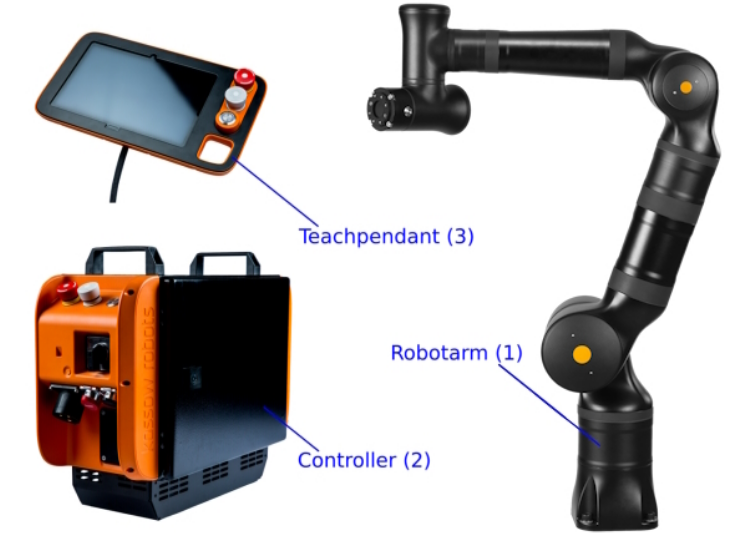
\includegraphics[width=0.5\textwidth]{figures/kassow-robot-parts.png}
    \caption{Functional parts of the KR collaborative robot (Source: \cite{kassow-manual})}
    \label{fig:kassow-robot-parts}
\end{figure}

The robotic arm comes with a robot controller and a teach pendant as shown in Figure \ref{fig:kassow-robot-parts} A robot controller is the main controlling unit for each \hyperref[acro:KR]{KR} manipulator.
Teach Pendant is used for programming the manipulator and also provides \hyperref[acro:UI]{UI} and safety controls. 
The robot can be operated manually and automatically. It is automated, programmable and capable of
moving in up to seven axes. The robot is typically used for welding, painting, assembly, pick and place,
packaging and labelling. These are all carried out while ensuring high endurance, speed, and precision. \cite[page 23]{kassow-manual}


\begin{table}[h!]
    \centering
    \small
    \renewcommand{\arraystretch}{1.2} % Adjusts row height
    \begin{tabular}{ll}
        \textbf{Description} & \textbf{Value} \\ \hline
        Type & Collaborative \\
        Reach & 1400 mm in all directions\\
        Number of axis & 7-axis \\
        Operating temperature range & 0-45°C\\ 
        Weight & 38.0 kg \\ 
        AC Power connector & 1 Phase CEE \\ 
        Typical Power consumption & 400-1200W \\ 
        Supply voltage & 100-120 and 200-240 VAC (50/60hz) \\ 
        Supply current & 16A\\ 
        \hyperref[acro:IO]{IO} power supply & 24 VDC\\ 
        Max. joint speed  & 163/225 °/s\\ 
        Max. static force on \hyperref[acro:TFC]{TFC} (payload) & 10 kg\\ 
        Max. static torque on \hyperref[acro:TFC]{TFC} & 25 Nm\\ 
        Sound level & Below 70dB (A) \\ 
        Ingress protection & IP54 \\ 
        Joint ranges & Joint 1,3,5,6,7 +/- 360° \\
        & Joint 2,4 -70/+180° \\ 
        Footprint& $160 \times 160$ mm \\ 
        ROS Support & Available \\ \hline
    \end{tabular}
    \caption{KR1410 Technical Specifications (Source: \cite[page 31]{kassow-specification})}
\end{table}


Kassow Robots can be integrated with other devices via Profinet. Each robot that is equipped with optional Profinet 
\hyperref[acro:HW]{HW} interface can act as a Profinet IO-Device.
This means that such robot can be monitored and controlled by any Profinet IO-Controller (for example PLC). \cite{profinet}
KR1410 could be also interfaced with ROS. KR provides packages to install through which KR messages communication is set up to a PC.
These messages are used to get the current joint configuration of the robot and simulate it in ROS or web UI.

KR also provides developmental environment to add new robotic peripherals, like grippers or sensors. This development environment is \hyperref[acro:CBun]{CBun},
which allows writing KR software in C++ for a specific peripheral. It is used in order to setup communication between VISOR camera functions and the robot. \cite{Cbun}
